\chapter{Analyse}
Die Umsetzung des Projekts erforderte vorerst eine genauere Analyse des Projekts. Es ergibt sich, dass das Projekt logisch in verschiedene Teilaspekte unterteilbar ist.

\section{Augmented Reality auf einem mobilen Telefon}
Die grundlegende Überlegung ist, die Realität auf einem Handy in der Art darzustellen, dass diese nachträglich beliebig erweiterbar ist. Dies geschieht beispielsweise durch das Einblenden von nur virtuell existenten Objekten. Dadurch wird dem Benutzer eine Erweiterung der eigentlichen Realität vorgetäuscht.
Die Realität wird hierfür durch die Kamera des mobilen Gerätes aufgefangen und verarbeitet. Für die nachträgliche Bearbeitung reicht es jedoch nicht, das Bild der Kamera in einer Live-View wiederzugeben. Stattdessen muss eine 3D-Umgebung existieren, die es ermöglicht, nicht existente Objekte in das Bild einzufügen.

\begin{figure}[!h]
  \centering
    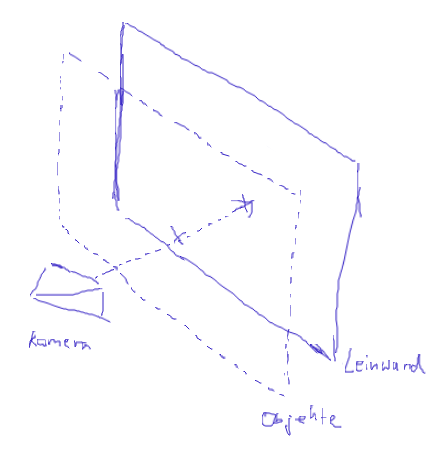
\includegraphics[width=8cm]{szene_skizze}
    \caption{Aufbau der AR-Szene}
    \label{fig:scene_sketch}
\end{figure}

Die Lösung ist eine simulierte Leinwand in einer 3D-Umgebung. Hierfür wird eine Fläche erstellt, die orthogonal zur Kamera steht. Diese Fläche wird mit dem Live-Bild der Kamera des mobilen Gerätes texturiert. Nun ist es möglich fremde Objekte in das Kamerabild einzufügen, indem man diese Objekte zwischen Leinwand und Kamera platziert.
Wichtig hierbei ist, dass die Leinwandfläche zu jeder Zeit orthogonal zur Blickrichtung der Kamera ist, da der Benutzer ansonsten den Abstand zwischen virtuellem Objekt und Leinwand sehen kann, wodurch die Illusion verloren geht. Ein weiteres Problem ist die Simulation von Tiefe auf diese Art und Weise. Die virtuellen Objekte stehen in der 3D-Umgebung in einem festen Abstand zur Leinwand. Wenn ein Objekt in der eigentlichen Realität nun weiter entfernt steht als ein anderes, muss die Tiefe durch eine Veränderung der Größe simuliert werden.

Um eine noch realistischere Darstellung der virtuellen Objekte zu ermöglichen, ist der Einsatz eines Virtual-Reality-Headsets möglich. Aufgrund der geringen Anschaffungskosten und der Kompatibilität zu vielen Mobilgeräten ist hierfür die Verwendung des Google Cardboard angedacht.

\section{Marker}
Ein genereller Ansatz zur Realisierung von Augmented Reality ist der Einsatz von Markern. Die Marker dienen als Stellvertreter von virtuellen Objekten in der Realität. Das Programm, welches Augmented Reality simulieren möchte, kann nun die Position und Orientierung der Marker durch Verarbeitung des Kamerabildes wahrnehmen, und virtuelle Objekte an dieser Stelle platzieren.
Eine wichtige Entscheidung ist die Wahl der Art des Markers. In diesem Projekt wurden sich für QR-Codes als Marker entschieden.
Bei dem QR-Code handelt es sich um ein weit verbreitetes Verfahren. Es existieren daher viele Bibliotheken, die das Verarbeiten von QR-Codes realisieren. Des weiteren ist das Erkennungs- und Leseverfahren für QR-Codes durch eine automatische Fehlerkorrektur sehr robust. Das ist wichtig, da die Auflösung des Kamerabildes für eine Live-Verarbeitung auf einem mobilen Gerät nicht zu hoch sein darf. Trotzdem müssen die Marker zuverlässig erkannt werden. Ein weiterer Vorteil ist, dass QR-Codes zusätzlich zur Position noch weitere Informationen im QR-Code selbst tragen können. Auf diese Weise ist es möglich, abhängig vom Marker verschiedene Inhalte einzublenden.

\section{Entwicklungsumgebung}
Bei der Wahl der Entwicklungsumgebung für mobile Anwendungen kann grundsätzlich zwischen zwei Ansätzen unterschieden werden. Zum einen kann nativ für eine Zielplattform entwickelt werden, zum anderen kann ein Framework oder eine Engine verwendet werden, die die Entwicklung abstrahiert. Beide Varianten bieten Vor- und Nachteile. Ausschlaggebende Kriterien sind die Effizienz, die Unterstützung für weitere externe Softwarekomponenten, die einfache Handhabung und mögliche Zielplattformen.

Ein Vorteil der nativen Entwicklung liegt in der Effizienz. Nur exakt die benötigten Komponenten sind in der finalen App vorhanden. Die Verwendung einer Engine führt häufig dazu, dass weitere, eigentlich ungenutzte, Abhängigkeiten die Dateigröße zusätzlich erhöhen, oder eine Auswirkung auf die Leistung haben.

Der große Vorteil in der Verwendung einer Engine liegt, darin, dass die Anwendung für unterschiedliche Zielplattformen veröffentlicht werden kann, ohne dass sie für jede Plattform von Grund auf neu entwickelt werden muss. Außerdem erleichtert eine Engine die Handhabung grafischer Funktionen, beispielsweise das Laden von 3D-Modellen und deren Positionierung im Raum.

Die Wahl der Entwicklungsumgebung fiel auf die 3D-Engine Unity. Zusätzlich zu den bereits genannten Vorteilen einer Engine unterstützt sie die Verwendung von Bibliotheken zur QR-Code-Erkennung (ZXing) und die Benutzung des VR-Headsets Google Cardboard. Zudem existieren viele Ressourcen, die die Einarbeitung in die Arbeit mit der Engine erleichtern.
